\documentclass[doc]{apa6}

\usepackage{amssymb,amsmath}
\usepackage{ifxetex,ifluatex}
\usepackage{fixltx2e} % provides \textsubscript
\ifnum 0\ifxetex 1\fi\ifluatex 1\fi=0 % if pdftex
  \usepackage[T1]{fontenc}
  \usepackage[utf8]{inputenc}
\else % if luatex or xelatex
  \ifxetex
    \usepackage{mathspec}
    \usepackage{xltxtra,xunicode}
  \else
    \usepackage{fontspec}
  \fi
  \defaultfontfeatures{Mapping=tex-text,Scale=MatchLowercase}
  \newcommand{\euro}{€}
\fi
% use upquote if available, for straight quotes in verbatim environments
\IfFileExists{upquote.sty}{\usepackage{upquote}}{}
% use microtype if available
\IfFileExists{microtype.sty}{\usepackage{microtype}}{}

% Table formatting
\usepackage{longtable, booktabs}
\usepackage{lscape}
% \usepackage[counterclockwise]{rotating}   % Landscape page setup for large tables
\usepackage{multirow}		% Table styling
\usepackage{tabularx}		% Control Column width
\usepackage[flushleft]{threeparttable}	% Allows for three part tables with a specified notes section
\usepackage{threeparttablex}            % Lets threeparttable work with longtable

% Create new environments so endfloat can handle them
% \newenvironment{ltable}
%   {\begin{landscape}\begin{center}\begin{threeparttable}}
%   {\end{threeparttable}\end{center}\end{landscape}}

\newenvironment{lltable}
  {\begin{landscape}\begin{center}\begin{ThreePartTable}}
  {\end{ThreePartTable}\end{center}\end{landscape}}

  \usepackage{ifthen} % Only add declarations when endfloat package is loaded
  \ifthenelse{\equal{\string doc}{\string man}}{%
   \DeclareDelayedFloatFlavor{ThreePartTable}{table} % Make endfloat play with longtable
   % \DeclareDelayedFloatFlavor{ltable}{table} % Make endfloat play with lscape
   \DeclareDelayedFloatFlavor{lltable}{table} % Make endfloat play with lscape & longtable
  }{}%



% The following enables adjusting longtable caption width to table width
% Solution found at http://golatex.de/longtable-mit-caption-so-breit-wie-die-tabelle-t15767.html
\makeatletter
\newcommand\LastLTentrywidth{1em}
\newlength\longtablewidth
\setlength{\longtablewidth}{1in}
\newcommand\getlongtablewidth{%
 \begingroup
  \ifcsname LT@\roman{LT@tables}\endcsname
  \global\longtablewidth=0pt
  \renewcommand\LT@entry[2]{\global\advance\longtablewidth by ##2\relax\gdef\LastLTentrywidth{##2}}%
  \@nameuse{LT@\roman{LT@tables}}%
  \fi
\endgroup}


  \usepackage{graphicx}
  \makeatletter
  \def\maxwidth{\ifdim\Gin@nat@width>\linewidth\linewidth\else\Gin@nat@width\fi}
  \def\maxheight{\ifdim\Gin@nat@height>\textheight\textheight\else\Gin@nat@height\fi}
  \makeatother
  % Scale images if necessary, so that they will not overflow the page
  % margins by default, and it is still possible to overwrite the defaults
  % using explicit options in \includegraphics[width, height, ...]{}
  \setkeys{Gin}{width=\maxwidth,height=\maxheight,keepaspectratio}
\ifxetex
  \usepackage[setpagesize=false, % page size defined by xetex
              unicode=false, % unicode breaks when used with xetex
              xetex]{hyperref}
\else
  \usepackage[unicode=true]{hyperref}
\fi
\hypersetup{breaklinks=true,
            pdfauthor={},
            pdftitle={Evaluating Content-Related Validity Evidence Using Text Modeling},
            colorlinks=true,
            citecolor=blue,
            urlcolor=blue,
            linkcolor=black,
            pdfborder={0 0 0}}
\urlstyle{same}  % don't use monospace font for urls

\setlength{\parindent}{0pt}
%\setlength{\parskip}{0pt plus 0pt minus 0pt}

\setlength{\emergencystretch}{3em}  % prevent overfull lines


% Manuscript styling
\captionsetup{font=singlespacing,justification=justified}
\usepackage{csquotes}
\usepackage{upgreek}



\usepackage{tikz} % Variable definition to generate author note

% fix for \tightlist problem in pandoc 1.14
\providecommand{\tightlist}{%
  \setlength{\itemsep}{0pt}\setlength{\parskip}{0pt}}

% Essential manuscript parts
  \title{Evaluating Content-Related Validity Evidence Using Text Modeling}

  \shorttitle{Text Modeling Validity}


  \author{Daniel Anderson\textsuperscript{1}, Brock Rowley\textsuperscript{1}, \& Sondra Stegenga\textsuperscript{1}}

  % \def\affdep{{"", "", ""}}%
  % \def\affcity{{"", "", ""}}%

  \affiliation{
    \vspace{0.5cm}
          \textsuperscript{1} University of Oregon  }

  \authornote{
    Correspondence concerning this article should be addressed to Daniel
    Anderson, 5262 University of Oregon. E-mail:
    \href{mailto:daniela@uoregon.edu}{\nolinkurl{daniela@uoregon.edu}}
  }


  \abstract{Topic modeling is applied with science content standards to evaluate
semantic clustering. The probability that each item from a statewide
assessment belongs to each cluster/topic is then estimated as a source
of content-related validity evidence. We also show how visualizations
can map the content coverage of the test.}
  




\usepackage{amsthm}
\newtheorem{theorem}{Theorem}[section]
\newtheorem{lemma}{Lemma}[section]
\theoremstyle{definition}
\newtheorem{definition}{Definition}[section]
\newtheorem{corollary}{Corollary}[section]
\newtheorem{proposition}{Proposition}[section]
\theoremstyle{definition}
\newtheorem{example}{Example}[section]
\theoremstyle{definition}
\newtheorem{exercise}{Exercise}[section]
\theoremstyle{remark}
\newtheorem*{remark}{Remark}
\newtheorem*{solution}{Solution}
\begin{document}

\maketitle

\setcounter{secnumdepth}{0}



(800 Words)

\hypertarget{conceptual-framework}{%
\subsection{Conceptual Framework}\label{conceptual-framework}}

The alignment of test items to content standards is critical to content
validity. Generally, alignment studies are used to determine content
validity for standards-based assessments. Alignment studies are
difficult to execute and design, even under ideal conditions, and
present researchers with potential sources of error. The chosen
methodology, number of participants, professional judgments, consensus
through discussion or averaged by ratings, costs associated with travel,
and time are elements for consideration. Text mining may be an
additional source of content validity, used to match content standards
to items for standards-based assessments.

\hypertarget{methods-and-results}{%
\subsection{Methods and Results}\label{methods-and-results}}

Data were analyzed using using R (R Core Team, 2017) with packages stm
(Roberts, Stewart, Tingley, Benoit, 2018), and tm (Feinerer, 2018) for
text mining and structural topic modeling. All plots were produced using
R (R Core Team, 2017) with the ggplot2 (Wickham, 2016). All code for
producing the different plots will be made available for the full
conference paper, including publicly available data that can be used for
fully reproducible examples.

\hypertarget{conclusions-and-implications}{%
\subsection{Conclusions and
Implications}\label{conclusions-and-implications}}

Overall, this paper will discuss a new and innovative proposed approach
to establishing validity through analyzing and categorizing text data
via modern data tools of R and RStudio text analysis and structural
topic modeling. It does not replace current methods for establishing
validity but demonstrates initial promise to add strength to the
development design. In a world of constantly evolving and growing data
and data sources it is imperative as educational researchers that we not
only begin to explore new methods that hold promise for increasing
efficiency and accuracy with data analysis but also ensure that methods
engage an element of translatability. By increasing the accuracy of
constructs and improved validity we provide the opportunity to increase
utility and translatability over a range of consumers in the educational
community. In addition, modern technology provides an array of methods
and open source resources and tools, such as R and RStudio, that not
only provide the ability to capture and categorize the data but also
visualize the findings. Again, this is an imperative piece in a world
that has seen vastly increased calls for the translation of data and
research to practice and practice to research.

\#\#References

Anderson, D. , Irvin, S. , Alonzo, J. and Tindal, G. A. (2015), Gauging
Item Alignment Through Online Systems While Controlling for Rater
Effects. Educational Measurement: Issues and Practice, 34: 22-33.
\url{doi:10.1111/emip.12038}

Meyer, David and Hornik, Kurt and Feinerer, Ingo (2008) Text Mining
Infrastructure in R. Journal of Statistical Software, 25 (5). pp.~1-54.
ISSN 1548-7660

R Core Team (2017). R: A language and environment for statistical
computing. R Foundation for Statistical Computing, Vienna, Austria. URL
\url{https://www.R-project.org/}.

Raudenbush, S. W., \& Willms, J. (1995). The estimation of school
effects. Journal of educational and behavioral statistics, 20(4),
307-335.

USCB (2017). Geographic Terms and Concepts - Census Tract. Retrieved
July 28, 2017 from
\url{https://www.census.gov/geo/reference/gtc/gtc_ct.html}

Walker, K. (2017). tidycensus: Load US Census Boundary and Attribute
Data as \enquote{tidyverse} and \enquote{sf}-Ready Data Frames. R
package version 0.1.2.
\url{https://CRAN.R-project.org/package=tidycensus}

Wickham, H. (2016). ggplot2: Elegant Graphics for Data Analysis.
Springer-Verlag New York, 2016.

Wilke, C. O. (2017). ggjoy: Joyplots in \enquote{ggplot2}. R package
version 0.2.0. \url{https://CRAN.R-project.org/package=ggjoy}

\hypertarget{tables-and-figures}{%
\subsection{Tables and Figures}\label{tables-and-figures}}

(No Limit)

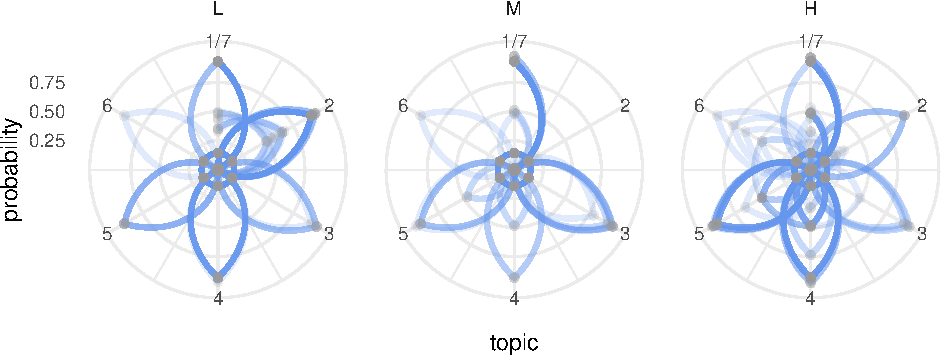
\includegraphics{ncme19_files/figure-latex/modeling-1.pdf}






\end{document}
